%=============================================================================
%
%	Optimization in Banach Spaces
%
%	Continuos evaluation work - Block 2
%
%=============================================================================



%=============================================================================
%	Packages
%=============================================================================

\documentclass[11pt, a4paper]{article}		% document format
\usepackage{graphicx}						% package to insert graphics
\usepackage[english]{babel}
\usepackage[utf8]{inputenc}					% this enables all unicode characters
\usepackage{amsmath, amsfonts, amssymb} 	% maths packages
\usepackage{amsthm}							% theorem styles
\usepackage{fancyhdr}						% package for headers, foot and margin notes
\usepackage{enumitem}						% allows to change the enumeration format in line
\usepackage{tikz}
\usepackage[
  top=2cm,
  bottom=2cm,
  left=3cm,
  right=2cm,
  headheight=17pt, % as per the warning by fancyhdr
  includehead,includefoot,
  heightrounded, % to avoid spurious underfull messages
]{geometry} 




%=============================================================================
%	Commands
%=============================================================================

\providecommand{\U}[1]{\protect\rule{.1in}{.1in}}
\newcommand{\N}{\mathbb{N}}
\newcommand{\E}{\mathcal{E}}
\newcommand{\R}{\mathbb{R}}



%=============================================================================
%	Environment
%=============================================================================

\theoremstyle{plain}
\newtheorem{theorem}{Theorem}%[section]
\newtheorem{lema}[theorem]{Lema}
\newtheorem{exercise}{Exercise}
\newtheorem{algorithm*}{Algorithm}

\theoremstyle{definition}
\newtheorem{solution}{Solution}[exercise]
\renewcommand*{\thesolution}{\theexercise.\alph{solution}}	% Make solution instances enumerate with number of exercise and letter of solution

\usetikzlibrary{calc}



%============================================================================
%	Pagestyle
%=============================================================================

\pagestyle{fancy}		% As we use the fancyhdr pkg need the fancy pagestyle, for more information:
						% http://tug.ctan.org/tex-archive/macros/latex/contrib/fancyhdr/fancyhdr.pdf


%\topmargin 0 pt
%\oddsidemargin 0 pt
%\evensidemargin 0 pt
%\marginparwidth 0 pt


%\textheight 25cm
%\textwidth 400 pt
%\advance\textheight by \topskip

%\parindent 0pt
%\parskip 5mm plus 1mm minus 1mm

\fancyhead[C]{PEC 2}					                	% Central header
\fancyhead[L]{Optimization in Banach Spaces}   				% Left header
\fancyhead[R]{Marc Jovani Bertran}						    % Right header



%=============================================================================
%	Document
%=============================================================================

\begin{document}
	\section*{1}

Sea $(X, \| \cdot \|)$ un espacio real normado, $f : X \rightarrow \R$ un funcional convexo y $x_0 \in X$.
\begin{enumerate}[label=(\alph*)]
    \item Pruebe que $\partial f(x_0)$ es un conjunto convexo (contenido en el conjunto de funcionales lineales continuos $l : X \rightarrow \R$). 
    \item Sea $x^*: X \rightarrow \R$ un funcional lineal y continuo. Pruebe que
        \begin{enumerate}[label=(\alph{enumi}.\arabic*)]
            \item $\partial (f + x^*)(x_0) = x^* + \partial f(x_0)$, 
            \item $\partial (\lambda f)(x_0) = \lambda \partial f(x_0)$.
        \end{enumerate}
\end{enumerate}

\noindent\rule{10cm}{0.4pt}


\subsection*{(a)}

Para probar (a) primero vemos que por el Teorema 3.26 del texto base como $f$ es convexo el conjunto $\partial f(x_0)$ es no vació.
Recordamos que la definición de $\partial f(x_0)$ es,
\begin{equation*}
    \partial f(x_0) = \{ l \in X^* | f(x) \geq f(x_0) + l(x - x_0),\; \forall x \in X \},
\end{equation*}
donde $X^*$ es el espacio dual de $X$.

Para todo $l_1, l_2 \in \partial f(x_0)$ y para todo $\lambda \in [0,1]$,
dado $x \in X$ tenemos,
\begin{equation*}
    (\lambda l_1 + (1 - \lambda) l_2) (x - x_0) = \lambda l_1 (x - x_0) + (1 - \lambda) l_2 (x - x_0).
\end{equation*}

Por tanto,
\begin{equation*}
\begin{aligned}
    f(x_0) + (\lambda l_1 + (1 - \lambda) l_2) (x - x_0) 
        & = f(x_0) + \lambda l_1 (x - x_0) + (1 - \lambda) l_2 (x - x_0) \\
        & = \lambda (f(x_0) + l_1 (x - x_0)) + (1 - \lambda) (f(x_0) + l_2 (x - x_0)) \\
        & \leq \lambda f(x) + (1 - \lambda) f(x) \\
        & = f(x). \\
\end{aligned}
\end{equation*}
Y por tanto $(\lambda l_1 + (1 - \lambda) l_2) \in \partial f(x_0)$, lo que implica que $\partial f(x_0)$ es convexo.


\subsection*{(b.1)}

Vemos que $\partial (f + x^*)(x_0) \subset x^* + \partial f(x_0)$.
Para todo $\l \in \partial (f + x^*)(x_0)$ tenemos que
\begin{equation*}
    (f + x^*)(x) \geq (f + x^*)(x_0) + l(x - x_0) 
    \Rightarrow f(x_0) \geq f(x_0) + l(x - x_0) - x^*(x - x_0) = f(x_0) + (l - x^*)(x - x_0),
\end{equation*}
dado que $x^*$ es un funcional lineal y continuo,
concluimos que $l - x^* \in \partial f(x_0)$ y esto implica que $l \in x^* + \partial f(x_0)$.

Veamos ahora que $x^* + \partial f(x_0) \subset \partial (f + x^*)(x_0)$.
Sea $l \in \partial f(x_0)$ entonces,
\begin{equation*}
    (f + x^*)(x_0) + (l + x^*)(x - x_0)
        = f(x_0) + l(x - x_0) + x^*(x_0) + x^*(x - x_0)
        \leq f(x) + x^*(x),
\end{equation*}
por tanto $l + x^* \in \partial (f + x^*)(x_0)$,
que implica $x^* + \partial f(x_0) \subset \partial (f + x^*)(x_0)$ y consecuentemente  $x^* + \partial f(x_0) = \partial (f + x^*)(x_0)$.


\subsection*{(b.2)}

Igual que en el apartado anterior comprobamos ambas inclusiones.
Veamos que $\partial (\lambda f)(x_0) \subset \lambda \partial f(x_0)$.
Para todo $l \in \partial (\lambda f)(x_0)$, tenemos
\begin{equation*}
    (\lambda f)(x) \geq (\lambda f)(x_0) + l(x - x_0) 
    \Rightarrow f(x) \geq f(x_0) + \frac{1}{\lambda} l(x - x_0),
\end{equation*}
por tanto $\frac{1}{\lambda} l \in \partial f(x_0)$ que implica $l \in \lambda \partial f(x_0)$.

Veamos ahora que $\lambda \partial f(x_0) \subset \partial (\lambda f)(x_0)$.
Sea $l \in \partial f(x_0)$ y sea $\lambda > 0$, entonces
\begin{equation*}
    \lambda f(x) \geq \lambda f(x_0) + \lambda l(x - x0),
\end{equation*}
por tanto $\lambda l \in \partial (\lambda f)(x_0)$.
Y se cumple $\partial (\lambda f)(x_0) = \lambda \partial f(x_0)$.

	\section*{2}

Sea $\| \cdot \|_{\diamond}$ una norma en $\R^n$ y sea
\begin{equation*}
    f(x) = \| x \|_{\diamond}.
\end{equation*}
Se define la norma dual del siguiente modo:
\begin{equation*}
    \| l \|_{*} 
        = \max_{h \neq 0} \frac{| \langle l, h \rangle |}{\| h \|_{\diamond}}
        = \max_{\| h \|_{\diamond} = 1} | \langle l, h \rangle |.
\end{equation*}
Pruebe que se cumplen las siguientes propiedades:
\begin{enumerate}[label=(\alph*)]
    \item $\partial f(0) = \{ l \in \R^n : \| l \|_{*} \leq 1 \}$. En particular, pruebe que
        \begin{enumerate}[label=(\alph{enumi}.\arabic*)]
            \item $\partial \| 0 \|_{2} = \{ l \in \R^n : \| l \|_{2} \leq 1 \}$,
            \item $\partial \| 0 \|_{1} = \{ l \in \R^n : \| l \|_{\infty} \leq 1 \}$,
            \item $\partial \| 0 \|_{\infty} = \{ l \in \R^n : \| l \|_{1} \leq 1 \}$,
        \end{enumerate}

    \item $\partial f(x) = \{ l \in \R^n : \| l \|_{*} \leq 1, \; \langle l, x \rangle = \| x \|_{\diamond} \}$,
        para cada $x \in \R^n$.
    
\end{enumerate}

\noindent\rule{10cm}{0.4pt}

\subsection*{(a)}

Aplicando la definición de subgradiente tenemos
\begin{equation*}
\begin{aligned}
    \partial \| 0 \|_{\diamond}
        & = \{ l \in \R^n : \| x \|_{\diamond} \geq l(x), \; \forall x \in \R^n \} \\
        & = \{ l \in \R^n : \frac{| l(x) |}{\| x \|_{\diamond}} \leq 1, \; \forall x \in \R^n \setminus \{ 0 \} \} \\
        & = \{ l \in \R^n : \| l \|_{*} \leq 1 \}. \\
\end{aligned}
\end{equation*}

Los siguientes subapartados son consecuencia del resultado anterior y que el dual de la norma $\ell^2$ es $\ell^2$,
el dual de $\ell^1$ es $\ell^\infty$ y el dual de $\ell^\infty$ es $\ell^1$.

\subsubsection*{Norma dual de $\ell^2$}

Para ver que la norma dual de $\ell^2$ es ella misma usamos la siguiente definición norma dual,
para cualquier $y \in (\R^n)^* = \R^n$,
\begin{equation*}
    \| y \|_{2}^{*} = \sup_{\| x \|_2 \leq 1} | \langle x, y \rangle |.
\end{equation*}
Usando la desigualdad de Cauchy-Schwarz tenemos,
\begin{equation*}
        | \langle x, y \rangle |
        \leq \| x \|_2 \| y \|_2
        \leq \| y \|_2,
\end{equation*},
donde en la ultima desigualdad usamos $\| x \| \leq 1$.
Finalmente si usamos $x = \frac{y}{\| y \|_2}$, que cumple $\| x \| = 1$,
tenemos
\begin{equation*}
    | \langle x, y \rangle | = \| y \|_2,
\end{equation*}
alcanzando el supremo y por tanto
\begin{equation*}
    \| y \|_{2}^{*} = \| y \|_2.
\end{equation*}

\subsubsection*{Norma dual de $\ell^\infty$}

Veamos que la norma dual de $\ell^\infty$ es $\ell^1$,
tenemos que para cualquier $y \in (\R^n)^* = \R^n$,
\begin{equation*}
    \| y \|_{\infty}^{*} = \sup_{\| x \|_\infty \leq 1} | \langle x, y \rangle |
        = \sup_{\max_{1 \leq i \leq n} |x_i| \leq 1} \left| \sum_{i = 1}^{n} x_i y_i \right|.
\end{equation*}
La restricción $\max_{1 \leq i \leq n} |x_i| \leq 1$,
implica que $x \in [-1, 1]^n \subset \R^n$.

Para maximizar la suma elegimos $x \in[-1, 1]^n$ tal que
\begin{equation*}
    x_i = \left\{
    \begin{aligned}
        1     & \text{ si } y_i \geq 0, \\
        -1    & \text{ si } y_i < 0.
    \end{aligned}
        \right.
\end{equation*}
De este modo se tiene
\begin{equation*}
    | \langle x, y \rangle | = \sum_{i = 1}^{n} |y_i|,
\end{equation*}
i por tanto
\begin{equation*}
    \| y \|_{\infty}^{*} = \sum_{i = 1}^{n} |y_i| = \| y \|_1.
\end{equation*}

\subsubsection*{Norma dual de $\ell^1$}

Finalmente veamos que la norma dual de $\ell^1$ es $\ell^\infty$,
tenemos que para cualquier $y \in (\R^n)^* = \R^n$,
\begin{equation*}
    \| y \|_{1}^{*} = \sup_{\| x \|_1 \leq 1} | \langle x, y \rangle |
        = \sup_{\sum_{i = 1}^{n} |x_i| \leq 1} \left| \sum_{i = 1}^{n} x_i y_i \right|.
\end{equation*}

Para maximizar $ | \langle x, y \rangle | $ con la restricción $\| x \|_1 \leq 1$,
los componente $|x_i|$ deberían estar concentrados en maximizar los valores mas grandes $|y_i$.
En particular el máximo se alcanza cuando $x_k = \text{signo}(y_k)$ para $|y_k|$ el componente mas grande de $y$ y $x_i = 0$ para todo $i \neq k$.
Esto es, sea $k = \text{argmax}_{1 \leq i \leq n} |y_i|$, entonces
\begin{equation*}
    x_i = \left\{
    \begin{aligned}
        \text{signo}(y_k)   & \text{ si } i = k, \\
        0                   & \text{ si } i \neq k.
    \end{aligned}
        \right.
\end{equation*}
En tal caso la norma dual es
\begin{equation*}
    \| y \|_{1}^{*} = \max_{1 \leq i \leq n} |y_i| = \| y \|_\infty.
\end{equation*}



\subsection*{(b)}

Veamos que 
\begin{equation*}
    \partial f(x) = \{ l \in \R^n : \| l \|_{*} \leq 1, \; \langle l, x \rangle = \| x \|_{\diamond} \}, \; \forall x \in \R^n,
\end{equation*}
en el caso $x = 0$, ya hemos visto en el apartado anterior que se cumple,
por tanto veamos que se cumple para $x \neq 0$.


Sea $l \in \R^n$ tal que $\| l \|_{*} \leq 1$ y $\langle l, x \rangle = \| x \|_{\diamond}$,
tenemos que para cualquier $y \in \R^n$,
\begin{equation*}
\begin{aligned}
    \| x \|_{\diamond} + \langle l, y - x \rangle
        & = \| x \|_{\diamond} + \langle l, y \rangle - \langle l, x \rangle \\
        & = \| x \|_{\diamond} + \langle l, y \rangle - \| x \|_{\diamond} \\
        & = \langle l, y \rangle \\ 
        & \leq \| y \|_{\diamond} \cdot \frac{|\langle l, y \rangle|}{\| y \|_{\diamond}} \\
        & \leq \| y \|_{\diamond} \| l \|_{*} \\
        & \leq \| y \|_{\diamond},
\end{aligned}
\end{equation*}
por tanto $l \in \partial \| x \|_{\diamond}$,
que implica $\{ l \in \R^n : \| l \|_{*} \leq 1, \; \langle l, x \rangle = \| x \|_{\diamond} \} \subset \partial f(x)$,
para todo $x \in \R^n$.

Sea $l \in \partial f(x)$,
tenemos que
\begin{equation*}
    \| x \|_{\diamond} - \langle l, x \rangle 
        = \| 2x \|_{\diamond} - \| x \|_{\diamond} - \langle l, 2x - x \rangle
        \geq 0,
\end{equation*}
y
\begin{equation*}
    - \| x \|_{\diamond} + \langle l, x \rangle 
        = \| 0 \|_{\diamond} - \| x \|_{\diamond} - \langle l, 0 - x \rangle
        \geq 0.
\end{equation*}
Las dos desigualdades llevan a $\| x \|_{\diamond} = \langle l, x \rangle$.
Ademas para todo $y \in \R^n$, se cumple
\begin{equation*}
\begin{aligned}
    \| y \|_{\diamond}
        & \geq \| x \|_{\diamond} + \langle l, y - x \rangle \\
        & = \| x \|_{\diamond} + \langle l, y \rangle - \| x \|_{\diamond} \\
        & = \langle l, y \rangle.
\end{aligned}
\end{equation*}
Por lo tanto podemos concluir que
\begin{equation*}
    \| l \|_{*} 
        = \sup_{y \in \R^n} \frac{|\langle l, y \rangle}{\| y \|_{\diamond}} 
        \leq 1.
\end{equation*}
Por tanto se cumple $\partial f(x) \subset \{ l \in \R^n : \| l \|_{*} \leq 1, \; \langle l, x \rangle = \| x \|_{\diamond} \}$, para todo $x \in \R^n$.
Y con ambas inclusiones concluimos que $\partial f(x) = \{ l \in \R^n : \| l \|_{*} \leq 1, \; \langle l, x \rangle = \| x \|_{\diamond} \}$.
	\section*{3}

Sean $f_1 , f_2 : \R^n \rightarrow \R$ dos funciones diferenciables y convexas. Se considera la función
\begin{equation*}
    f (x) = \max \{f1 (x), f2 (x)\}.
\end{equation*}
Sea $x_0 \in \R^n$ un punto tal que $f (x_0) = f_1 (x_0) = f_2 (x_0)$.
Pruebe que $l$ es un subgradiente de $f$ en $x_0$ si y sólo si
\begin{equation*}
    l = \lambda \nabla f_1 (x_0) + (1 - \lambda) \nabla f_2 (x_0), \text{ para } \lambda \in [0, 1]. 
\end{equation*}

\noindent\rule{10cm}{0.4pt}

Supongamos que $l$ es de la forma
\begin{equation*}
    l = \lambda \nabla f_1 (x_0) + (1 - \lambda) \nabla f_2 (x_0),
\end{equation*}
con $\lambda \in [0, 1]$.
Entonces
\begin{equation}\label{ex3_ineq}
\begin{aligned}
    f(x_0) + l(x - x_0)
        & = f(x_0) + \lambda \nabla f_1 (x_0) (x - x_0) + (1 - \lambda) \nabla f_2 (x_0) (x - x_0) \\
        & \leq f(x_0) + \lambda (f_1(x) - f_1(x_0)) + (1 - \lambda) (f_2(x) - f_2(x_0)) \\
        & = \lambda f_1(x) + (1 - \lambda) f_2(x) \\
        & \leq f(x),
\end{aligned}
\end{equation}
donde en la primera desigualdad hemos usado el Lema 3.3 del texto base para ver que
\begin{equation*}
    \nabla g (\hat{x}) (x - \hat{x}) \leq g(x) - g(\hat{x}),
\end{equation*}
para toda función $g$ convexa.
Y la desigualdad $(\ref{ex3_ineq})$ confirma que $l \in \partial f(x_0)$.

La idea para ver que todo subgradiente es de la forma
\begin{equation*}
    l = \lambda \nabla f_1 (x_0) + (1 - \lambda) \nabla f_2 (x_0), \text{ para } \lambda \in [0, 1],
\end{equation*}
es porque en el punto $x_0$ dado que las dos funciones coinciden sus dos vectores tangentes se cruzan en $x_0$,
en cada dirección dominara uno u otro en función de si $f_1$ o $f_2$ es mayor que la otra en un pequeño entorno de $x_0$.
Si el subgradiente no esta comprimido entre los dos vectores tangentes entonces en algún punto no se cumplirá la desigualdad $f(x) \geq f(x_0) + l(x - x_0)$.
La Figura \ref{ex3_plot} ilustra esta idea en una dimension.

\begin{figure}[h]
\centering
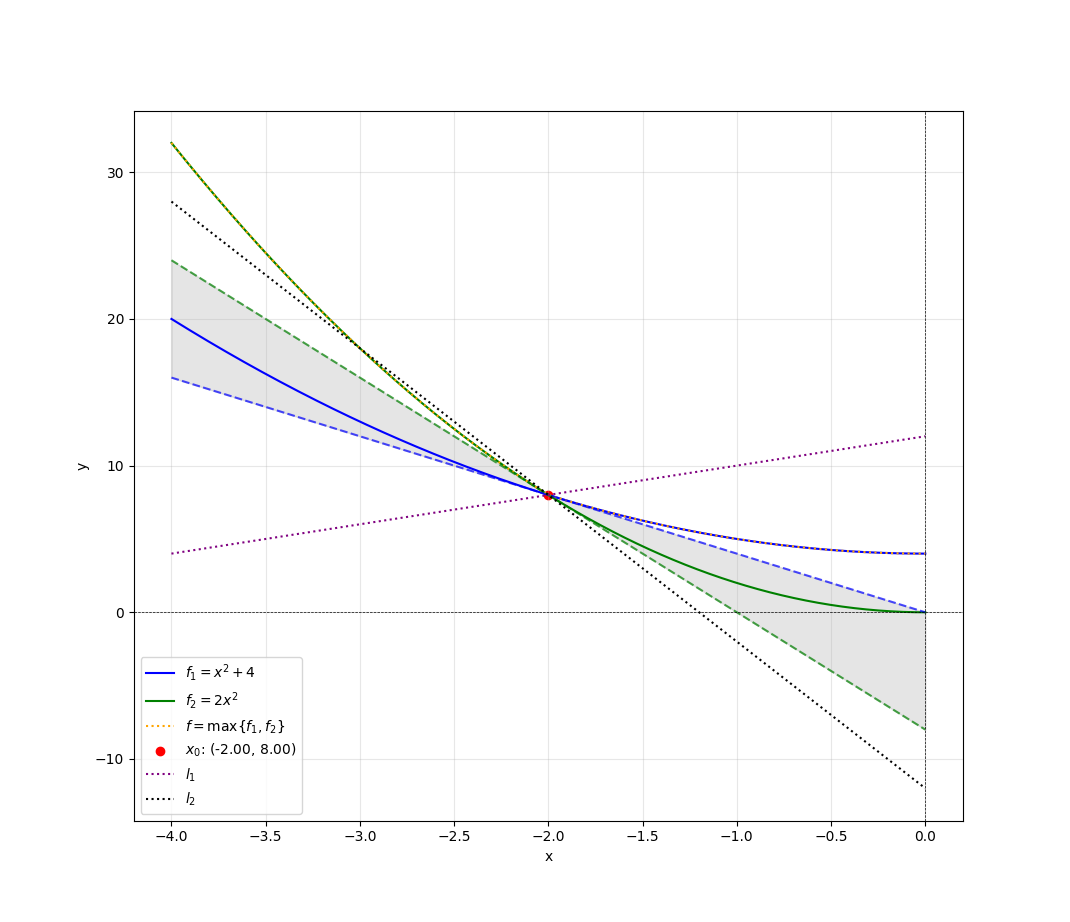
\includegraphics[scale=0.6]{ex3_plot.png}
\caption{
    El gráfico muestra dos funciones convexas y su máximo,
    el area gris es el area comprimida entre los dos vectores tangentes,
    y $l_1, l_2$ son dos vectores que pasan por $x_0$ pero no están en el area gris,
    se ve como no cumplen la desigualdad.
}
\label{ex3_plot}
\end{figure}

Vamos a formalizar la idea.
Sea $l \in \partial f(x_0)$ tal que
\begin{equation*}
    l \neq l_{\lambda} = \lambda \nabla f_1 (x_0) + (1 - \lambda) \nabla f_2 (x_0), \text{ para } \lambda \in [0, 1].
\end{equation*}
Entonces existe $h \in \R^n$ tal que
\begin{equation*}
    l(h) > l_{\lambda}(h), \forall \lambda \in [0, 1] \Rightarrow
    \left\{
    \begin{aligned}
        l(h) > \nabla f_1(x_0)(h), \\
        l(h) > \nabla f_2(x_0)(h). \\
    \end{aligned}
    \right.
\end{equation*}
Sin perdida de generalidad podemos suponer que para un $\alpha > 0$ suficientemente pequeño para que se cumpla
\begin{equation*}
    f(x_0 + \beta h) = f_1(x_0 + \beta h) \geq f_2(x_0 + \beta h), \; \forall 0 \leq \beta \leq \alpha.
\end{equation*}
Y por tanto en la dirección $h$ la derivada direccional de $f$ se corresponde con el gradiente de $f_1$,
\begin{equation*}
    f'(x_0)(h) = \nabla f_1(x_0)(h).
\end{equation*}
Entonces por el Lema 3.25 del texto base tenemos que
\begin{equation*}
    f'(x_0)(h) = \nabla f_1(x_0)(h) \geq l(h) !!
\end{equation*}
que contradice $l(h) > \nabla f_1(x_0)(h)$ y por tanto contradice $l \neq l_{\lambda}$.
Resultando en que $\exists \lambda \in [0,1]$ tal que $l = l_{\lambda}$, como queríamos ver.

	\section*{4}

Sea $(X, \| \cdot \|)$ un espacio real normado y $f : X \rightarrow \R := \R \cup \{-\infty, +\infty\}$.
La función $f^* : X^* \rightarrow \R$ definida por
\begin{equation*}
    f^* (x^*) = \sup_{x \in X} \{ \langle x, x^* \rangle - f(x) \},
\end{equation*}
se denomina la conjugada de Fenchel de $f$ ($X^*$ denota el conjunto de funcionales lineales y continuos $l : X \rightarrow \R$).

\begin{enumerate}[label=(\alph*)]
    \item Pruebe que
        \begin{equation*}
            f(x) + f^* (x^*) \geq \langle x, x^* \rangle, \quad \forall x \in X, \quad x^* \in X^*.
        \end{equation*}
        La desigualdad anterior se conoce como \textit{desigualdad de Young-Fenchel}.
    
    \item Sea $x_0 \in \text{dom} f$. Demuestre que
        \begin{equation*}
            x^* \in \partial f(x_0)
        \end{equation*}
        si y sólo si
        \begin{equation}\label{ex4_eq1}
            f(x) + f^*(x^*) = \langle x_0, x^* \rangle,
        \end{equation}
        y que lo anterior implica que $x_0 \in \partial f^*(x^*)$.
    
    \item Sea $x_0 \in \text{dom} f$. Demuestre que
        \begin{equation*}
            \partial f(x_0) \neq \emptyset 
                \iff f(x_0) = \max_{x^* \in X^*} (\langle x_0, x^* \rangle - f^*(x^*)).
        \end{equation*}
    
\end{enumerate}

\noindent\rule{10cm}{0.4pt}

\subsection*{(a)}

Para cualquier $x \in X$ y $x^* \in X^*$, tenemos
\begin{equation*}
\begin{aligned}
    f(x) + f^*(x^*)
        & = f(x) + \sup_{\hat{x} \in X} \{ \langle \hat{x}, x^* \rangle -f(\hat{x}) \} \\
        & \geq f(x) + \langle x, x^* \rangle - f(x) \\
        & = \langle x, x^* \rangle.
\end{aligned}
\end{equation*}
Como queríamos ver.


\subsection*{(b)}

Supongamos que $x^* \in \partial f(x_0)$,
entonces,
\begin{equation*}
\begin{aligned}
    f(x) & \geq f(x_0) + \langle x - x_0, x^* \rangle, \; \forall x \in X, \\
    & \Rightarrow \langle x_0, x^* \rangle \geq f(x_0) + \{ \langle x, x^* \rangle - f(x) \} , \; \forall x \in X, \\
    & \Rightarrow \langle x_0, x^* \rangle \geq f(x_0) + f^*(x^*). \\
\end{aligned} 
\end{equation*}
Usando el anterior resultado junto al resultado del apartado anterior,
tenemos que
\begin{equation*}
    \langle x_0, x^* \rangle = f(x_0) + f^*(x^*).
\end{equation*}

Supongamos ahora que $x^*$ cumple $(\ref{ex4_eq1})$,
entonces para todo $x \in X$, tenemos
\begin{equation*}
\begin{aligned}
    f(x_0) + \langle x - x_0, x^* \rangle
        & = \langle x, x^* \rangle - \langle x_0, x^* \rangle + \langle x_0, x^* \rangle - f^*(x^*) \\
        & = \langle x, x^* \rangle - \sup_{\hat{x} \in X} \{ \langle \hat{x}, x^* \rangle -f(\hat{x}) \} \\
        & \leq \langle x, x^* \rangle - (\langle x, x^* \rangle - f(x))  \\
        & = f(x),  \\
\end{aligned}
\end{equation*}
por tanto $x^* \in \partial f(x_0)$.

Finalmente veamos que si $x^* \in X^*$ y $x_0 \in X$ cumplen $(\ref{ex4_eq1})$,
entonces se tiene que para cualquier $y^* \in X^*$
\begin{equation*}
\begin{aligned}
    f^*(x^*) + \langle x_0, y^* - x^* \rangle
        & = - f(x_0) + \langle x_0, x^* \rangle - \langle x_0, x^* \rangle + \langle x_0, y^* \rangle \\
        & = \langle x_0, y^* \rangle - f(x_0) \\
        & \leq \sup_{x \in X} \{ \langle x, y^* \rangle - f(x) \} \\
        & = f^*(y^*), \\
\end{aligned}
\end{equation*}
por tanto $x_0 \in \partial f^*(x^*)$.


\subsection*{(c)}

Supongamos que $\partial f(x_0) \neq \emptyset$ y que $y^* \in \partial f(x_0)$,
por la desigualdad de Young-Fenchel tenemos que
\begin{equation*}
    f(x_0) \geq \langle x_0, x^* \rangle - f^*(x^*), \; \forall x^* \in X^*,
\end{equation*}
lo que implica que
\begin{equation}\label{ex4_c_eq}
\begin{aligned}
    f(x_0) 
        & \geq \max_{x^* \in X^*} (\langle x_0, x^* \rangle - f^*(x^*)) \\
        & \geq \langle x_0, y^* \rangle - f^*(y^*) \\
        & = f(x_0), \\
\end{aligned}
\end{equation}
donde en la ultima igualdad hemos usado el resultado del apartado anterior.
Por tanto las desigualdades de $(\ref{ex4_c_eq})$ son igualdades y tenemos
\begin{equation*}
        f(x_0) = \max_{x^* \in X^*} (\langle x_0, x^* \rangle - f^*(x^*)).
\end{equation*}

Supongamos ahora que
\begin{equation*}
        f(x_0) = \max_{x^* \in X^*} (\langle x_0, x^* \rangle - f^*(x^*)).
\end{equation*}
Sea $y^* \in X^*$ tal que
\begin{equation*}
    \langle x_0, y^* \rangle - f^*(y^*) \geq \langle x_0, x^* \rangle - f^*(x^*),
\end{equation*}
es decir $y^*$ es un máximo de la función $\langle x_0, x^* \rangle - f^*(x^*)$.
Entonces tenemos que
\begin{equation*}
    f(x_0) + f^*(y^*) = \langle x_0, y^* \rangle,
\end{equation*}
por tanto usando el resultado del apartado anterior tenemos que $y^* \in \partial f(x_0)$,
y por tanto $\partial f(x_0) \neq \emptyset$.


\end{document}